\documentclass[9pt,twocolumn,twoside]{../../styles/osajnl}
\usepackage{fancyvrb}
\usepackage{listings}
\journal{i524} 

\title{Charge Detection Mass Spectrometry}

\author[1,*]{Scott McClary}

\affil[1]{School of Informatics and Computing, Bloomington, IN 47408, U.S.A.}

\affil[*]{Corresponding authors: scmcclar@indiana.edu}

\dates{project-001, \today}

\ociscodes{Chemistry, Cloud, Hadoop Streaming, HPC, I524, Parallel
  Computing}
\doi{\url{https://github.com/cloudmesh/sp17-i524/blob/master/project/S17-IO-3011/report/report.pdf}}

\begin{abstract}
A Charge Detection Mass Spectrometry research application, developed
at Indiana University by the Martin F. Jarrold research group, is used
to indicate the performance and simplicity benefits of using Cloudmesh
and Ansible Galaxy to deploy and run big data software on one or more
virtual machines in the cloud. This proprietary research application
was initially installed and run by hand on local servers and remote
Supercomputers. The research application performed well on these
powerful systems; however, the manual process of deploying and running
the application turned out to be inefficient and too cumbersome for
the domain scientists. Therefore, Cloudmesh and Ansible Galaxy were
leveraged in order to automate the deployment of virtual clusters and
execution of this research application in the cloud. This modification
abstracted away the need for explicit human interaction while
maintaining an efficient, reproducible and scalable Charge Detection
Mass Spectrometry research workflow.
\newline
\end{abstract}

\setboolean{displaycopyright}{true}

\begin{document}

\maketitle

\section{Introduction} \label{introduction}
\subsection{Research Background} \label{research-background}
The Martin F. Jarrold research group at Indiana University studies
Charge Detection Mass Spectrometry (CDMS) \cite{www-mfj}. Their
general day-to-day workflow consists of conducting many scientific
experiments using a Mass Spectrometer. This expensive scientific
instrument creates raw frequency data at a rate of four (4) MB/s
throughout the duration of each experiment. The research group has
developed a Fast Fourier based application written in Fortran to
processes this raw frequency data. The Fortran application generates
human interpretable output, which assists the domain scientists in
understanding the substances analyzed in the aforementioned
experiments. The outputted results contain detailed mass information
of the many ions discovered, which is used to solve important research
topics such as the measurement and classification of the Hepatitis B
virus. The mass and the abundance of the ions discovered by the
application can be plotted to determine \emph{Intermediates} that
exist between definitive peaks in the plot, shown in Figure
\ref{fig:hbvassembly}. This mass information can also be used to
generate two and three-dimensional graphical representations of the
ions, which help the domains scientists visualize the underlying
structure of the Hepatitis B virus, shown in Figure
\ref{fig:hbvassembly}.

\begin{figure}[h]
\centering
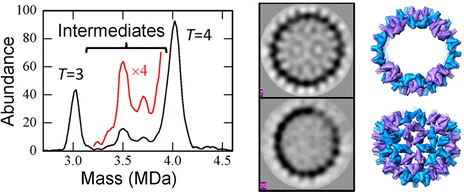
\includegraphics[height=1.35in, width=3.3in]{images/hbvassembly}
\caption{The chart to the left displays an accurate measurement of the
  Hepatitis B virus (HBV) created by the research group
  \cite{chem14cdms}. This detailed mass information is used to create
  the images shown in the middle and to the right, which show 2-D and
  3-D models of ions within the HBV. \cite{chem14cdms}}
\label{fig:hbvassembly}
\end{figure}

\subsection{General Problem} \label{problem}
The Martin F. Jarrold research group has the ability to generate a lot
of raw data, all of which needs to be processed by their Fortran
application, as shown in Figure \ref{fig:pipeline}. A typical day
conducting research consists of eight (8) to ten (10) one (1) hour
experiments with each experiment generating raw frequency data at a
rate of four (4) MB/s. Therefore, a single day of experiments has the
ability to generate up to one hundred and forty four (144) GB of
data. The research group must be able to process this data in a
similar amount of time as the time required to generate the raw
data. If their collection of compute resources is not powerful enough,
they will quickly become inundated with piles and piles of raw
data. This day-to-day research workflow typically strains the research
group's local compute resources. Furthermore, the research group
frequently makes algorithmic changes to the CDMS research
application. When a significant change occurs, the research group must
conduct a bulk reprocessing of months or even years worth of raw
data. When a bulk reprocess is required, the limited compute resources
available to the group become a significant limitation to the
efficiency of their research. Additionally, when the application is
run on remote systems, the raw input data must be transferred to the
remote systems and the resulting output must be aggregated and then
plotted in order to visualize and interpret the results. The process
of moving data around by hand is time consuming and the process to
aggregating results is tedious.

\subsection{General Solution} \label{solution}
The research group is composed of domain scientists who do not
necessarily have backgrounds in Computer Science
\cite{www-mfjgroup}. Therefore, a simple (i.e. automated) and
reproducible solution must be developed in order to satisfy their
day-to-day research workflow and their bulk reprocessing requirements.

\subsubsection{Cloud Computing}
Leveraging virtual clusters in the cloud to conduct their CDMS
analysis increases their available compute power while simultaneously
removing the need to explicitly manage a collection of compute
resources. Furthermore, the ability to dynamically scale up or down
the number of virtual machines aligns well with the evolving compute
needs of the research group. The software tools Cloudmesh Client and
Ansible Galaxy are at the foundation of this cloud computing solution
\cite{www-ansible-galaxy, www-cloudmesh}. These two software tools
collectively provide the ability to abstract away the technological
details of the deployment and installation of virtual clusters in the
cloud as well as automate the execution of the CDMS research
application. These general modifications to their research workflow
will ensure scalability, simplicity and reproducibility. These
improvements allow the domain scientists in the Martin F. Jarrold
research group to spend the majority of their time, effort and money
on their research and not on the technological challenges of running
the CDMS application.

\begin{figure}
\centering
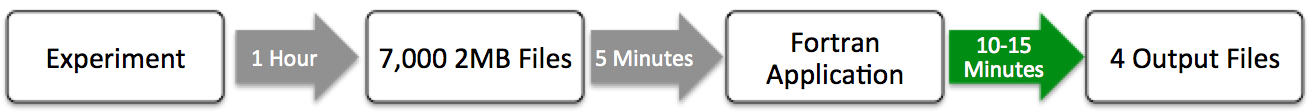
\includegraphics[height=0.45in, width=3.3in]{images/pipeline}
\caption{The Martin F. Jarrold research group's pipeline is shown
  above. This pipeline includes a one (1) hour experiment, which
  creates approximately seven thousand (7,000) two (2) MB raw
  frequency files. Each of these files need to be transferred to the
  remote compute resource(s) and processed with a Fortran application
  to generate four (4) human interpretable output files.}
\label{fig:pipeline}
\end{figure}

\begin{figure*}[h]
\centering
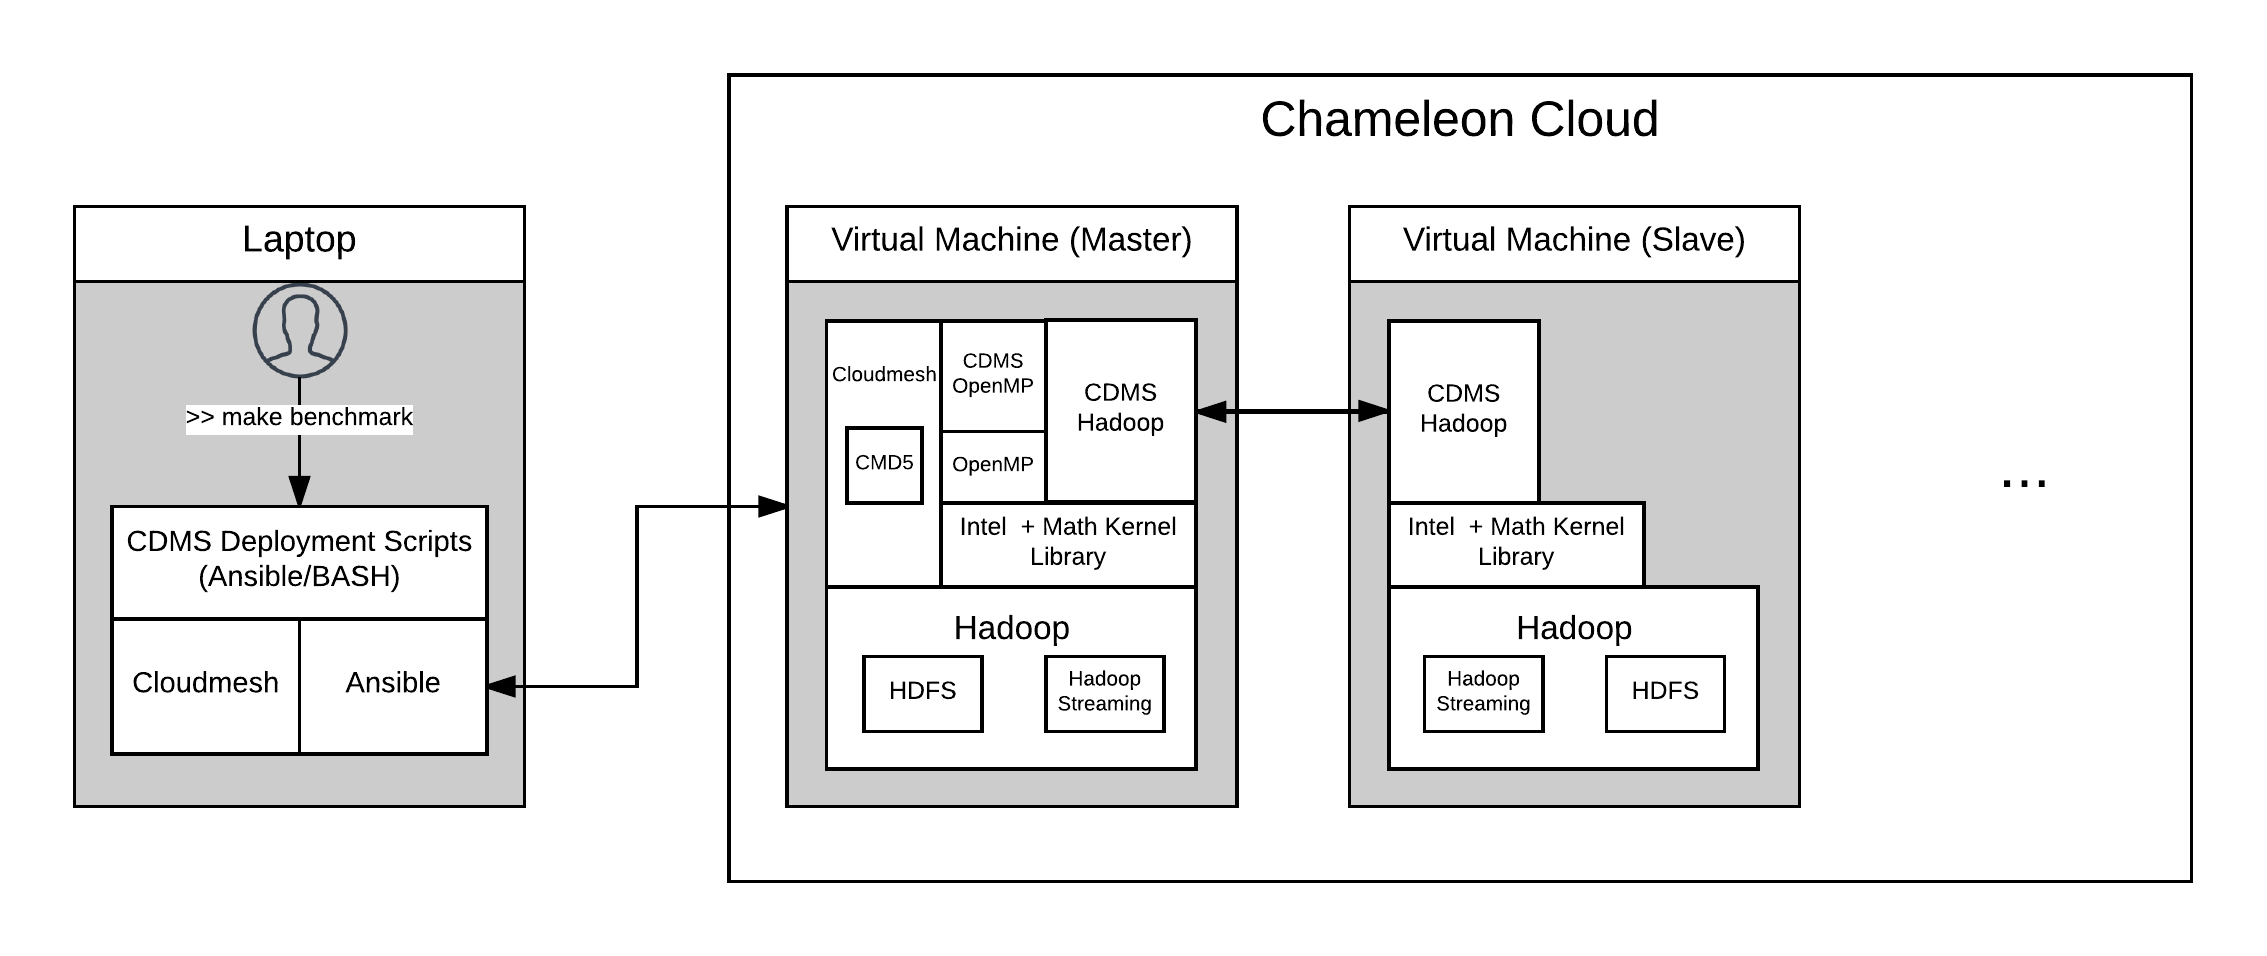
\includegraphics[height=3.0in, width=\textwidth]{images/architecture}
\caption{The figure above provides a visual representation of the
  underlying architecture required for the Charge Detection Mass
  Spectrometry Cloud Computing workflow. The necessary software
  (i.e. Cloudmesh, Ansible, Hadoop, Intel, and etc.) and compute
  resources (i.e. Laptop and Virtual Machines) are explicitly shown
  above.}
\end{figure*}

\section{Architecture} \label{architecture}
The underlying architecture of this cloud computing research workflow
is explicitly designed to facilitate automation. Cloudmesh and Ansible
Galaxy are software tools that enable the creation of a virtual
cluster, facilitate the deployment of software/data and automate the
execution of the CDMS research application.

\subsection{Software} \label{software}
\subsubsection{Cloudmesh Client Toolkit} 
The Cloudmesh Client Toolkit provides an application programming
interface (API), which allows users to simply manage a set of cloud
resources (i.e. virtual machines, virtual clusters and etc.)
\cite{www-cloudmesh}. The Cloudmesh Client Toolkit abstracts away the
technological details of managing cloud computing resources.

\subsubsection{Ansible Galaxy} 
Ansible is an information technology automation service designed for
software deployment and execution \cite{www-ansible}.  Ansible Galaxy
is an Ansible community, which ``provides pre-packaged units of work
known to Ansible as roles'' \cite{www-ansible-galaxy}. Ansible
Galaxy's pre-packaged units of work are essentially shared solutions
to common automation tasks. This is a representation of the open
source style of the Ansible Galaxy community. Ansible Galaxy promotes
fast development since the wheel does not need to be reinvented for
the automation of common tasks.

\subsubsection{CDMS Application} \label{cdms-app}
The Martin F. Jarrold Group has written a Fast Fourier based
application written in Fortran in order to conduct their CDMS
research. This application is composed of approximately fifteen
thousand (15,000) lines of Fortran code. Depending on the input, about
60\% to 70\% of the total compute time is spent within the external
Intel Math Kernel Library (MKL) conducting the required Fast Fourier
Transformations (FFT) \cite{www-intel-mkl}.

\subsubsection{Intel} 
The CDMS source code is compiled with the Intel compiler
\cite{www-intel}. The CDMS application relies on the Math Kernel
Library (MKL) to leverage efficient Fast Fourier Computations
\cite{www-intel-mkl}. The application also leverages the Intel OpenMP
parallel framework in order to divide the work amongst available CPU's
\cite{www-openmp}. Therefore, the Intel software is a fundamental
piece of the architecture, which provides the compiler, MKL, and
OpenMP functionality.

\subsubsection{Hadoop} 
Apache Hadoop ``is a framework that allows for the distributed
processing of large data sets across clusters of computers using
simple programming models'' \cite{www-hadoop}. Therefore, Hadoop must
be installed at the foundation of each virtual machine in the cloud in
order to leverage multiple virtual machines during the CDMS processing
phase of the workflow shown in Figure \ref{fig:pipeline}.

\subsection{Data} \label{data}
The CDMS application requires a set of raw two (2) MB files as
input. In order to develop and test the efficiency of the deployment,
a small dataset was used to generate all of the performance
results. This small test dataset, composed of two hundred (200) files
has a total size of four hundred (400) MB and is a representative
sample. A typical dataset for the research group is approximately
fourteen (14) GB in size. In a single day, up to ten (10) datasets are
created and need to be processed.

\section{Licensing} \label{licensing}
\subsection{CDMS Deployment Scripts} \label{source-license}
The source code (i.e. Bash, Ansible, Python) presented here is
licensed under the Apache License, Version 2.0 \cite{www-apache-lic}.

\subsection{CDMS Application} \label{cdms-license}
The Martin F. Jarrold Group research group owns all of the rights to
the Fortran Source code and data \cite{www-mfj}. All distribution of
the application and data must be consented by the research group.

\subsection{Intel} \label{intel-license}
The Intel software requires a license in order to complete the
installation \cite{www-intel-lic}. A student license is obtainable for
free with an \emph{EDU} email address; however, the leveraging the
Indiana University Intel license server would provide a more complete
and reproducible solution. In order to use the Indiana University
Intel license server, the Virtual Machines must reside in the Indiana
University IP address space. This can be achieved by connecting each
virtual machine to Indiana University's Virtual Private Network
(i.e. VPN) \cite{www-iu-vpn}. In order to connect to the VPN, one must
connect via DUO Authentication (i.e. use a phone or token to validate)
\cite{www-iu-duo}. Given the complexity and reliability concerns with
connecting to Indiana University's VPN simultaneously on multiple
virtual machines, the Intel software is activated with the free Intel
student license in order to promote simplicity and reproducibility.

\subsubsection{Student License Limitations} \label{student-license}
The CDMS Deployment Scripts that were developed for this project
leverage a free Intel student license to compile and link the CDMS
application. While anyone can use this student license, it is
registered to the author of this paper. This student license is
\emph{System Locked} and therefore can be installed on at most five
(5) virtual machines. Once this threshold has been passed, the Intel
software (i.e. compiler, MKL and OpenMP) can no longer be
activated. This limitation somewhat inhibits the reproducibility and
scalability of the research workflow. If a license registration error
occurs during the Intel build phase of the deployment of the software,
please contact the author of this paper. The author has the ability to
uninstall the license from the currently registered hosts using
Intel's Registration Center \cite{www-intel-reg}.

\section{Parallelization} \label{parallel}
The Charge Detection Mass Spectrometry input data is split into many
two (2) MB files. Conveniently, the data within each file is entirely
independent to the data in the other input files. Therefore, the input
data files can be processed simultaneously (i.e. in
parallel). Parallel processing may not seem important when working on
our sample dataset composed of two hundred (200) files; however, when
a large collection of data requires reprocessing, parallel processing
becomes critical to the efficiency of the Martin F. Jarrold research
group.
\subsection{OpenMP} \label{openmp-code}
OpenMP is a shared memory parallelization framework that is specified
with simple compiler directives \cite{www-openmp}. The shared memory
parallelization structure limits the scalability of the application to
a single node or virtual machine. This is in contrast to distributed
memory parallelization, such as Message Passing Interface (MPI) or
Hadoop, which enables multi-node parallelization \cite{www-mpi,
  www-hadoop}. The original developers of the CDMS application decided
to leverage OpenMP parallelization in order to exploit the natural
data independency and improve overall performance of the
application. However, this design choice limited the parallelization
(i.e. scalability) to a single node or virtual machine.

\subsection{Hadoop}
In order to improve the overall performance and scalability, a
distributed processing framework such as Hadoop must be integrated
into the foundation of the CDMS application. Such an enhancement would
allow for parallelization across multiple virtual machines. As
discussed in Section \ref{cdms-app}, the source code is composed of
fifteen thousand (15,000) lines of legacy Fortran code that interfaces
with the Intel Math Kernel Library. In order to leverage the Hadoop
MapReduce framework, the source code would need to be rewritten in a
compatible programming language such as Java or Python.

\subsubsection{Hadoop Streaming}
Hadoop Streaming provides an alternative to rewriting the application
in a compatible programming language. Hadoop Streaming allows one to
``create and run Map/Reduce jobs with any executable or script as the
mapper and/or the reducer'' \cite{www-hadoop-streaming}. In Hadoop
Streaming, ``the mapper and the reducer are executables that read the
input from stdin (line by line) and emit the output to stdout''
\cite{www-hadoop-streaming}. The CDMS application is designed to read
and write data to local files on disk; therefore, source code
modifications were required in order to ensure the application read
from stdin and wrote to stdout. The overall structure of the
application and its data, which is naturally split into many
relatively small files, allowed for a straightforward transformation
from OpenMP parallelization Hadoop Streaming parallelization, as shown
in Figure \ref{fig:hadoop}. Altering the way in which data was
inputted to and outputted from the CDMS application was the only
modification that was required in order to integrate Hadoop Streaming
parallelization.

\begin{figure}[h]
\centering
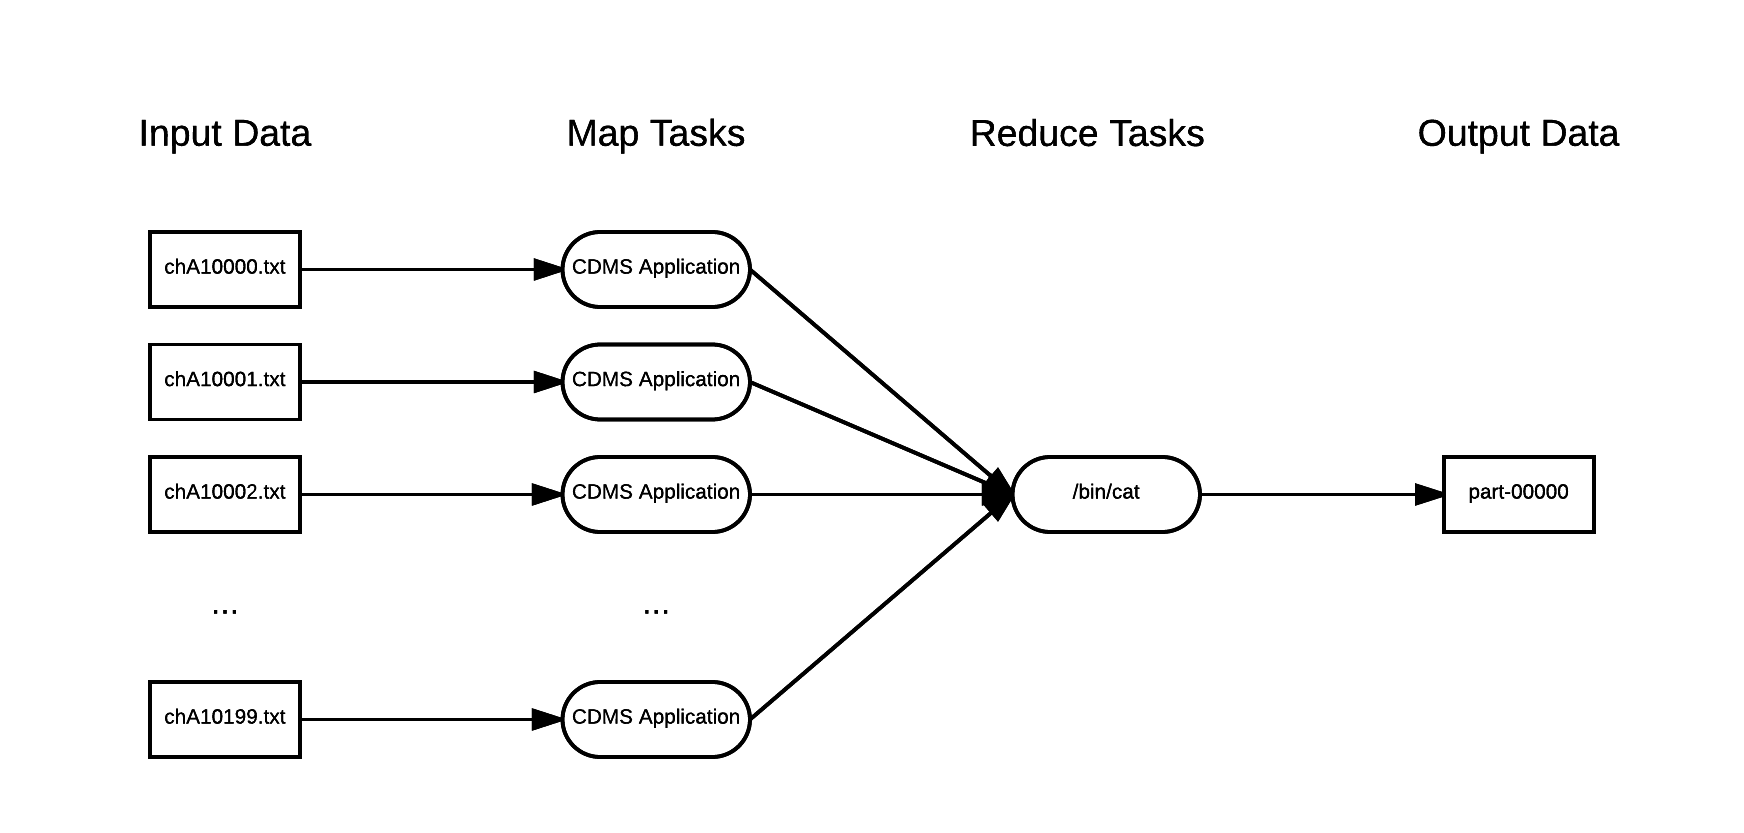
\includegraphics[height=1.65in, width=\columnwidth]{images/mapreduce}
\caption{The diagram shown above indicates the MapReduce style
  analysis of the CDMS Hadoop Streaming version of the
  application. Each two (2) MB input file is processed independently
  by the CDMS application and the results are aggregated with a single
  \emph{cat} reduce task.}
\label{fig:hadoop}
\end{figure}

\section{Getting Started}
The CDMS Deployment Scripts were specifically designed to promote
simplicity and reproducibility. The following subsections describe how
to use the CDMS Deployment Scripts to install and run the CDMS
application in the cloud with as little as one simple command.

\subsection{Requirements} \label{req}
In order to execute the CDMS Deployment Scripts, one must have the
Cloudmesh Client installed and configured on their local system. This
includes having a valid $\sim$/.cloudmesh/cloudmesh.yaml configuration
file, registering Chameleon as the default cloud, registering a
profile, uploading a ssh key and uploading a secgroup.

\subsection{Fetch Code} \label{git}
The CDMS Deployment Scripts are hosted using GitHub
\cite{www-github}. A single repository contains the required Ansible
and Bash scripts used to launch the CDMS research workflow
\cite{www-github-i524}.
\noindent See the following Bash commands:
\begin{lstlisting}[language=bash]
  >> git clone [REPOSITORY]
  >> cd sp17-i524/project/S17-IO-3011/code
\end{lstlisting}

\subsection{Benchmark} \label{benchmark-info}
A single command will deploy the Hadoop virtual cluster, install the
required software, run the three versions (i.e. Serial, OpenMP and
Hadoop Streaming) of the CDMS application, aggregate the results,
create plots of the output and delete the Hadoop virtual
cluster. Timing information for each of these stages is printed to the
screen once the benchmark has completed. The performance of this
benchmark is plotted and explained in Section \ref{performance}.
\noindent See the following Bash command:
\begin{lstlisting}[language=bash]
  >> make benchmark
\end{lstlisting}
By default the benchmark will be run on a virtual cluster containing a
single virtual machine. You can modify the maximum number of virtual
machines to be used in the benchmark by passing in an optional
argument to the \emph{benchmark} Makefile option. The example shown
below will run the entire benchmark with one, two and three virtual
machines.
\noindent See the following Bash command:
\begin{lstlisting}[language=bash]
  >> make benchmark num_nodes=3
\end{lstlisting}

\subsection{Additional Commands} \label{other}
In case one would like to break up the aforementioned benchmark into
individual pieces, there are separate Bash commands available.
\noindent See the following Bash commands:
\begin{lstlisting}[language=bash]
  >> make deploy [num_nodes=n]
  >> make install
  >> make run
  >> make view
  >> make delete
  >> make clean
\end{lstlisting}

\subsubsection{Deploy}
The \emph{deploy} Makefile option leverages Cloudmesh Client to deploy
a Hadoop virtual cluster in the Chameleon Cloud
\cite{www-chameleon}. By default one (1) virtual machines will be
created with the \emph{deploy} option. The specific number of virtual
machines deployed can be configured by passing in num\_nodes=n, where
n is the number of virtual machines requested to be deployed in the
virtual cluster.

\subsubsection{Install}
The \emph{install} Makefile option installs necessary software
(i.e. Intel Compiler, Intel MKL, Python, Pip, Cloudmesh, Git, Charge
Detection Mass Spectrometry application, and etc.) on the master and
slave virtual machines of the active virtual cluster.

\subsubsection{Run}
The \emph{run} Makefile option runs the serial, OpenMP, and Hadoop
Streaming versions of the CDMS application on the active virtual
cluster using the small test dataset containing two hundred (200)
input files.

\subsubsection{View}
The \emph{view} Makefile option aggregates the output data from the
virtual machines in the active cluster, plots the results using
Python's matplotlib and transfers a subset of the plots to the local
system in order to visually validate the accuracy of the application
\cite{www-matplotlib}.

\subsubsection{Delete}
The \emph{delete} Makefile option deletes all of the virtual machines
associated with active virtual cluster.

\subsubsection{Clean}
The \emph{clean} Makefile option removes all of the local output
files, if any exist.

\section{Compute Resources} \label{resources}
The CDMS OpenMP parallel version application was tested on multiple
compute resources, as explained in Section \ref{performance}. Each
resource has unique architectural qualities that impact the
performance, scalability and degree of parallelism. While the degree
of parallelism (i.e. number of CPUs) may not be indicative of
application performance, it certainly provides a baseline
understanding of some architectural differences amongst the four (4)
available systems.

\subsection{Windows HPC Server}
The Martin F. Jarrold's local Windows HPC Server has eight (8) CPUs;
therefore, the Charge Detection Mass Spectrometry OpenMP version
application can process up to eight (8) input files in parallel.

\subsection{Karst}
Indiana University's Linux Supercomputer, named Karst, has sixteen
(16) CPUs per node; therefore, the Charge Detection Mass Spectrometry
application can process up to sixteen (16) input files in parallel
\cite{www-karst}.

\subsection{Big Red II}
Indiana University's Linux Supercomputer, named Big Red II, has
thirty-two (32) CPUs per node; therefore, the Charge Detection Mass
Spectrometry OpenMP application can process up to thirty-two (32)
input files in parallel \cite{www-br2}.

\subsection{Chameleon Cloud}
The Cloudmesh Client allows one to specify different flavors of
virtual machines to be deployed in the Chameleon Cloud
\cite{www-cloudmesh, www-chameleon}. These flavors come in various
sizes (i.e. Memory, vCPUs, and etc.). As shown in Table
\ref{tab:hadoop}, these flavors can be used strategically to specify
the number of virtual CPUs allocated to each virtual machine. As an
example, the Chameleon Cloud m1.xlarge flavor provides eight (8)
vCPUs. This allows the Charge Detection Mass Spectrometry OpenMP
application to process up to eight (8) input files in
parallel. Additionally, the virtual machines deployed in the Chameleon
Cloud are running version 14.04 of the Ubuntu operating system.
\begin{table}[htbp]
\centering
\begin{tabular}{cc}
\multicolumn{2}{c}{\bf Chameleon Cloud Virtual Machine
  Flavors}\\ \hline \# Flavor & \# of vCPUs \\ \hline m1.medium & 2
\\ m1.large & 4 \\ m1.xlarge & 8 \\ \hline
\end{tabular}
\caption{The table above indicates the number of virtual CPUs
  allocated to the various virtual machine flavors in the Chameleon
  Cloud \cite{www-chameleon}. The number of vCPUs indicates the
  maximum degree of parallelism for the CDMS application.}
\label{tab:hadoop}
\end{table}

\section{Performance Results} \label{performance}
The following subsections describe the performance of the OpenMP and
Hadoop Streaming versions of the application. These performance
results only include the time-to-solution of the application
processing the two hundred (200) input files. Perforamnce results
including the entire deployment, installation and execution will be
explained in Section \ref{benchmark-performance}.

\subsection{OpenMP Scalability} \label{omp-scalability}
As discussed in Section \ref{openmp-code}, the application was
initially parallelized using OpenMP. This version of the application
attempts to utilize the computational power available on a single node
or virtual machine. Figure \ref{fig:scalability2} compares the
time-to-solution performance of the OpenMP version of the application
on the available compute resources (i.e. local servers, Supercomputers
and clouds) introduced in Section \ref{resources}. As expected the
time-to-solution (i.e. execution time) of the CDMS OpenMP version of
the application decreases as amount of compute resources increase, as
shown in Figure \ref{fig:scalability2}. For instance, on Karst the
application running with sixteen (16) OpenMP threads completes in
9.4\% of the time required for the application running with one (1)
OpenMP thread.

The application performs most efficiently on Karst when using sixteen
(16) CPUs (i.e. OpenMP threads). However, when the application is run
using one (1), two (2), four (4) or eight (8) CPUs, the best
performance exists on the Chameleon Cloud, as shown in Figure
\ref{fig:scalability2}. Specifically, the application performs 18\%
faster on a single Chameleon Cloud virtual machine when compared to
running the application on eight (8) CPUs of Karst.
\begin{figure}[h]
\centering
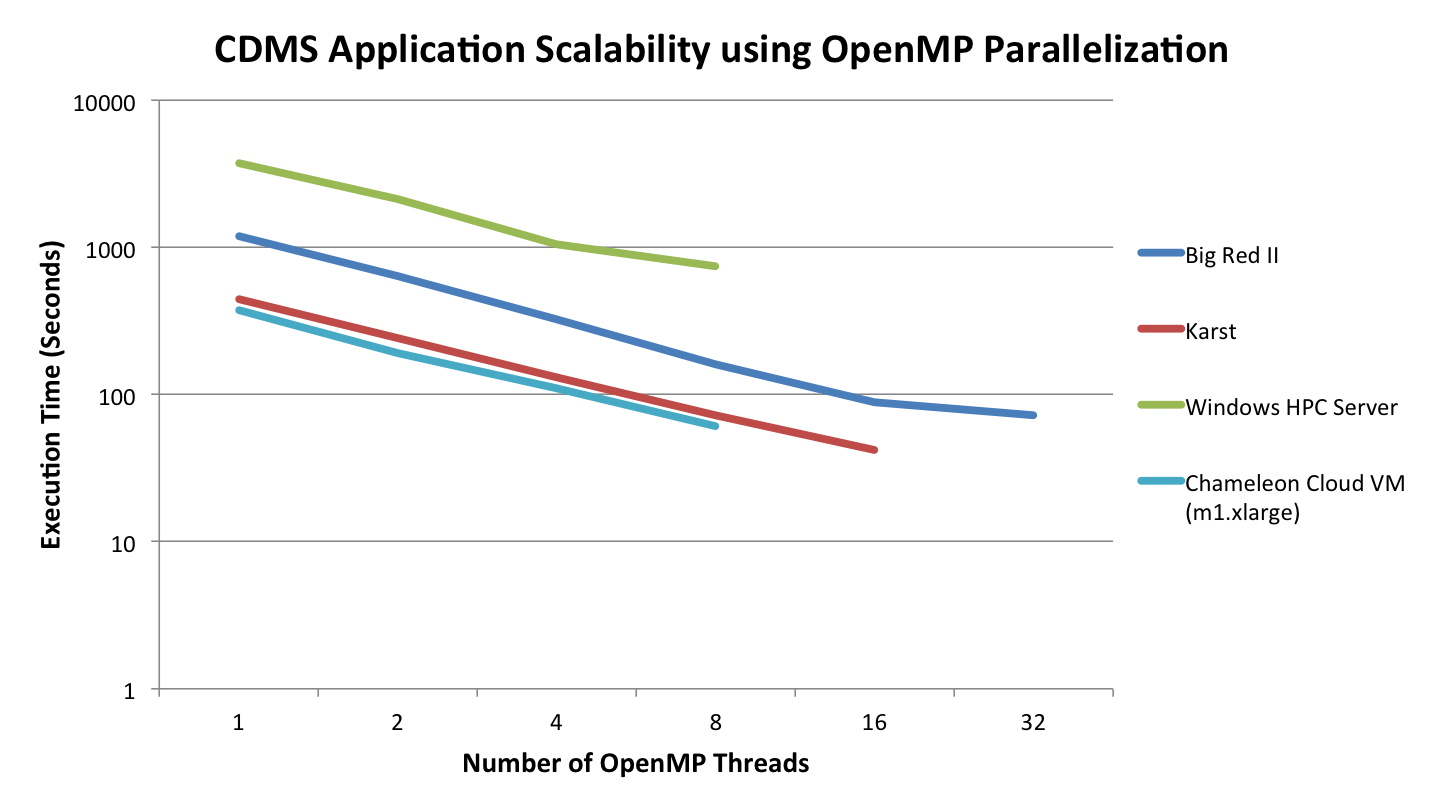
\includegraphics[height=2.1in, width=3.3in]{images/scalability2}
\caption{The figure above shows the scalability (i.e. reduction in
  time-to-solution) as the number of OpenMP threads increase on local
  servers, Supercomputers and Clouds.}
\label{fig:scalability2}
\end{figure}

\subsection{Hadoop Streaming Scalability} \label{hadoop-scalability}
Unfortunately, the performance results for the Hadoop Streaming
version of the CDMS application are not as promising as the
performance results for the OpenMP version of the application. The
Hadoop Streaming application does not exhibit the desired
scalability. Since the application is essentially a map only Hadoop
application, the performance (i.e. total runtime) of the application
should decrease linearly as the number of virtual machines
increase. However, the performance results shown in Figure
\ref{fig:hadoop-benchmark} indicate that the execution time remains
relatively consistent when one (1), two (2) or three (3) virtual
machines are used to process the two hundred (200) raw input
files. Interestingly, the performance of the application significantly
increases as the flavor of the virtual machine changes from smaller
(i.e. less vCPUs) to larger (i.e. more vCPUs). Figure
\ref{fig:hadoop-benchmark} shows that the Hadoop Streaming version of
the application run on a m1.xlarge flavor requires only 43\% of the
execution time as the same application run on a m1.medium flavor.

\begin{figure}[h]
\centering
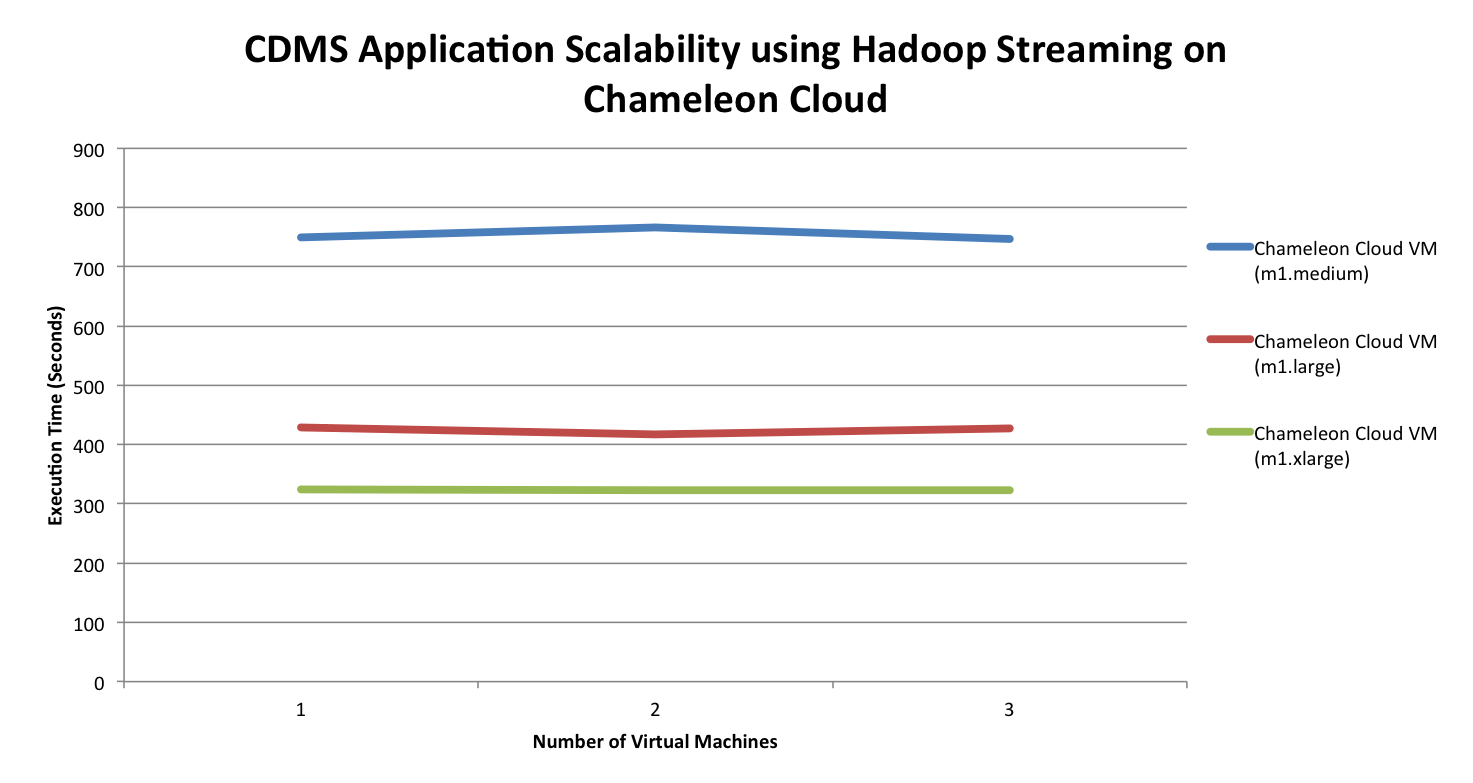
\includegraphics[height=2.1in, width=3.3in]{images/hadoop_benchmark}
\caption{The image above shows the scalability (i.e. reduction in
  time-to-solution) of the Charge Detection Mass Spectrometry Hadoop
  Streaming version of the application in a Chameleon Cloud virtual
  cluster. The performance information includes timing results for
  three (3) different virtual machine flavors.}
\label{fig:hadoop-benchmark}
\end{figure}

\subsection{Benchmark Scalability} \label{benchmark-performance}
The benchmark including the deployment of the virtual cluster,
installation of the required software, execution the
serial/OpenMP/Hadoop Streaming versions of the CDMS application and
the aggregation of the results was tested using one (1), two (2) and
three (3) virtual machines in the Chameleon Cloud. Interestingly, this
benchmark required increasing time as the number of virtual machines
increased, as shown in Figure \ref{fig:benchmark}. This performance
information indicates that the deployment overhead outweighs the
potential benefits of leveraging multiple virtual machines. The lack
of scalability shown in the Hadoop Streaming version of the
application and the small dataset are major factors, which contribute
to the overall performance results. Specifically, if the Hadoop
Streaming version of the application exhibited linear scalability and
the dataset was significantly larger, the overhead incurred would not
be as impactful as shown in Figure \ref{fig:benchmark}.

\begin{figure}[h]
\centering
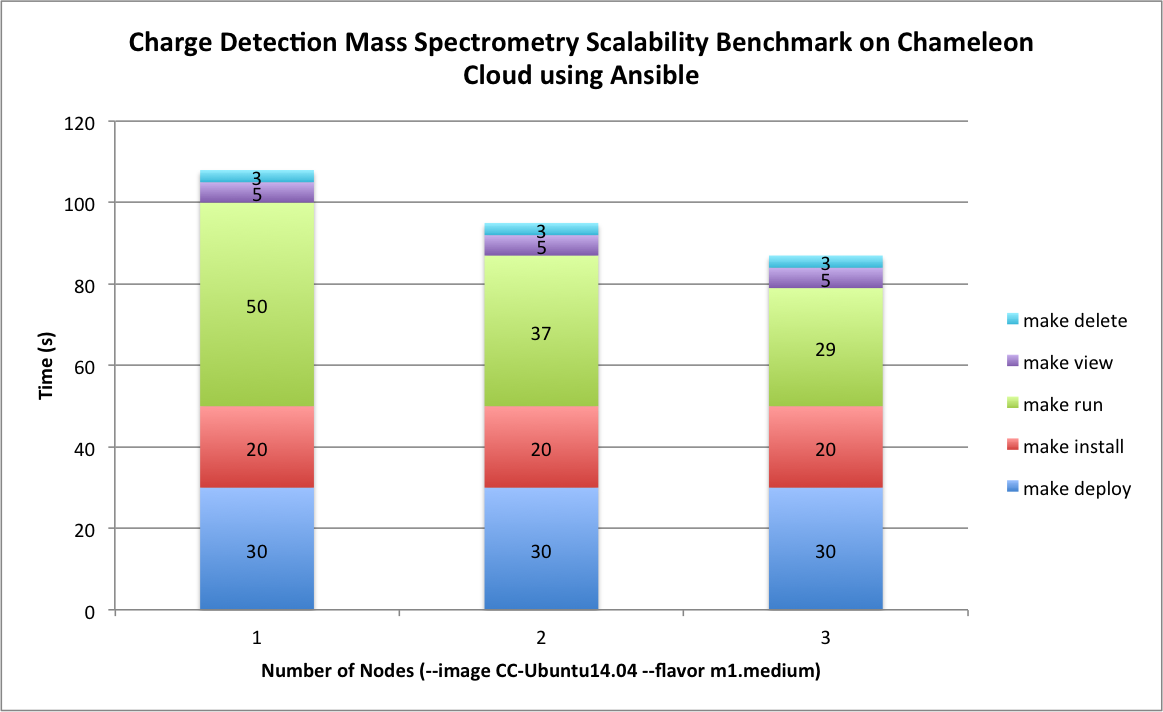
\includegraphics[height=2.1in, width=3.3in]{images/benchmark}
\caption{The figure above indicates the time-to-solution for a full
  benchmark of the deployment of one (1), two (2) and three (3)
  virtual machines in the Chameleon Cloud. This benchmark includes
  depoying the virtual machines, installing all of the software,
  running the serial, OpenMP and Hadoop Streaming versions of the
  application and aggregating/plotting the results.}
\label{fig:benchmark}
\end{figure}


\section{Future Work} \label{future}
Future work includes analyzing the performance of the CDMS Hadoop
Streaming application to understand the poor scalability when running
on a virtual cluster containing multiple virtual machines. Once the
scalability issue has been fixed, larger flavors and more virtual
machines will be utilized in order to increase the performance of the
Hadoop Streaming application.

Future work includes figuring out how to leverage Indiana University's
Intel license server. This will increase reproducibility by allowing
the Intel Compiler and Intel MKL to be installed on an unlimited
number of virtual machines.

Future work includes dispersing the raw input data across multiple
virtual machines and running an instance of the CDMS OpenMP version of
the application on each virtual machine and then aggregating the
results. This modification will increase scalability for the shared
memory parallelization.

Future work includes integrating Message Passing Interface (MPI) as
the parallelization structure of the application rather than OpenMP or
Hadoop Streaming \cite{www-mpi}. This will allow for a dramatic
increase in the scalability of the application.

\section{Conclusion} \label{conclusion}
The use of the Cloudmesh Client and Ansible Galaxy software to
automate the execution of the Charge Detection Mass Spectrometry
research application in the cloud improved the simplicity, efficiency
and reproducibility. The automation allows the Martin F. Jarrold
research group to focus on the details of their specific research
rather than on the details of managing the software subsystems,
executing the application and managing the input/output data. This
automated cloud computing solution benefits the Martin F. Jarrold
research group with respect to both simplicity and performance of the
application. Streamlining the research workflow will inevitably result
in an increase in productivity for the research group. An increase in
research productivity may also result in an increase in grant funding
and/or an increase in publications for the Indiana University research
group.

The performance of the CDMS OpenMP version of the application
performed favorably on a single Chameleon Cloud virtual machine when
compared with a single node of the Indiana University High Performance
Computing clusters (e.g. Karst and Big Red II). This unexpected result
has sparked future work in optimizing the OpenMP version of the
application for the Chameleon Cloud. However, the overhead included
with deploying the virtual cluster and installing the necessary
software causes the overall time-to-solution to increase dramatically.

The Hadoop Streaming version of the CDMS application did not exhibit
optimal performance on a Chameleon Cloud virtual cluster. If the
execution time reduced when more virtual machines were used, then this
version of the application would become a viable solution for the
research group's need to bulk reprocess raw input data. The Hadoop
streaming version of the CDMS application is a step in the right
direction; however, additional work must to be done to ensure
scalability across multiple virtual machines.

\section{Execution Plan} \label{plan}
The following subsections act as a timeline regarding how the project
was divided up in order to complete all of the work by the desired
deadline. The project execution plan is simply a guide and was
followed diligently; however, some items were pushed slightly forwards
or backwards as technological challenges were faced.
\subsection{March 6, 2017 - March 12, 2017}
This week I installed Cloudmesh on my local machine, created my first
virtual machine on the Chameleon Cloud and tested Ansible Galaxy on
remote systems such as one or more Chameleon Cloud virtual machine. I
also wrote the project proposal, which eventually became this project
report.
\subsection{March 13, 2017 - March 19, 2017}
This week I tested the deployment of the Intel Compiler on one or more
Chameleon Cloud virtual machine using Cloudmesh and Ansible
Galaxy. Given that I was out of town for Spring Break, I did not
expect significant progress to be made during this week.
\subsection{March 19, 2017 - March 26, 2017}
This week I attempted to configure the Intel Compiler and Math Kernel
Library to use the Indiana University Intel license server. Using this
license server required connecting to Indiana University's Virtual
Private Network (VPN) and using Two-Step Login (Duo) from the command
line.
\subsection{March 27, 2017 - April 2, 2017}
This week I deployed the Charge Detection Mass Spectrometry research
application along with the required input data on one or more
Chameleon Cloud virtual machines using Cloudmesh and Ansible Galaxy.
\subsection{April 3, 2017 - April 9, 2017}
This week I modified the source code of the OpenMP parallel Charge
Detection Mass Spectrometry research application to leverage Hadoop
Streaming.
\subsection{April 10, 2017 - April 16, 2017}
This week I benchmarked the Charge Detection Mass Spectrometry
research workflow on the Chameleon Cloud. This included varying the
number and size of the virtual machines. I also wrote Python scripts
to aggregate and plot the CDMS application's output from one or more
virtual machines and locally visualize the results.
\subsection{April 17, 2017 - April 23, 2017}
This week I ensured the reproducibility of my source code as well as
wrote and revised the final version of this report.


\section*{Acknowledgements}
The authors would like to thank the School of Informatics and
Computing for providing the Big Data Software and Projects (INFO-I524)
course \cite{www-i524}. This project would not have been possible
without the technical support \& edification from Gregor von Laszewski
and his distinguished colleagues.

 
\section*{Author Biographies}
\begingroup
\setlength\intextsep{0pt}
\begin{minipage}[t][3.2cm][t]{1.0\columnwidth} 
  \begin{wrapfigure}{L}{0.25\columnwidth}
    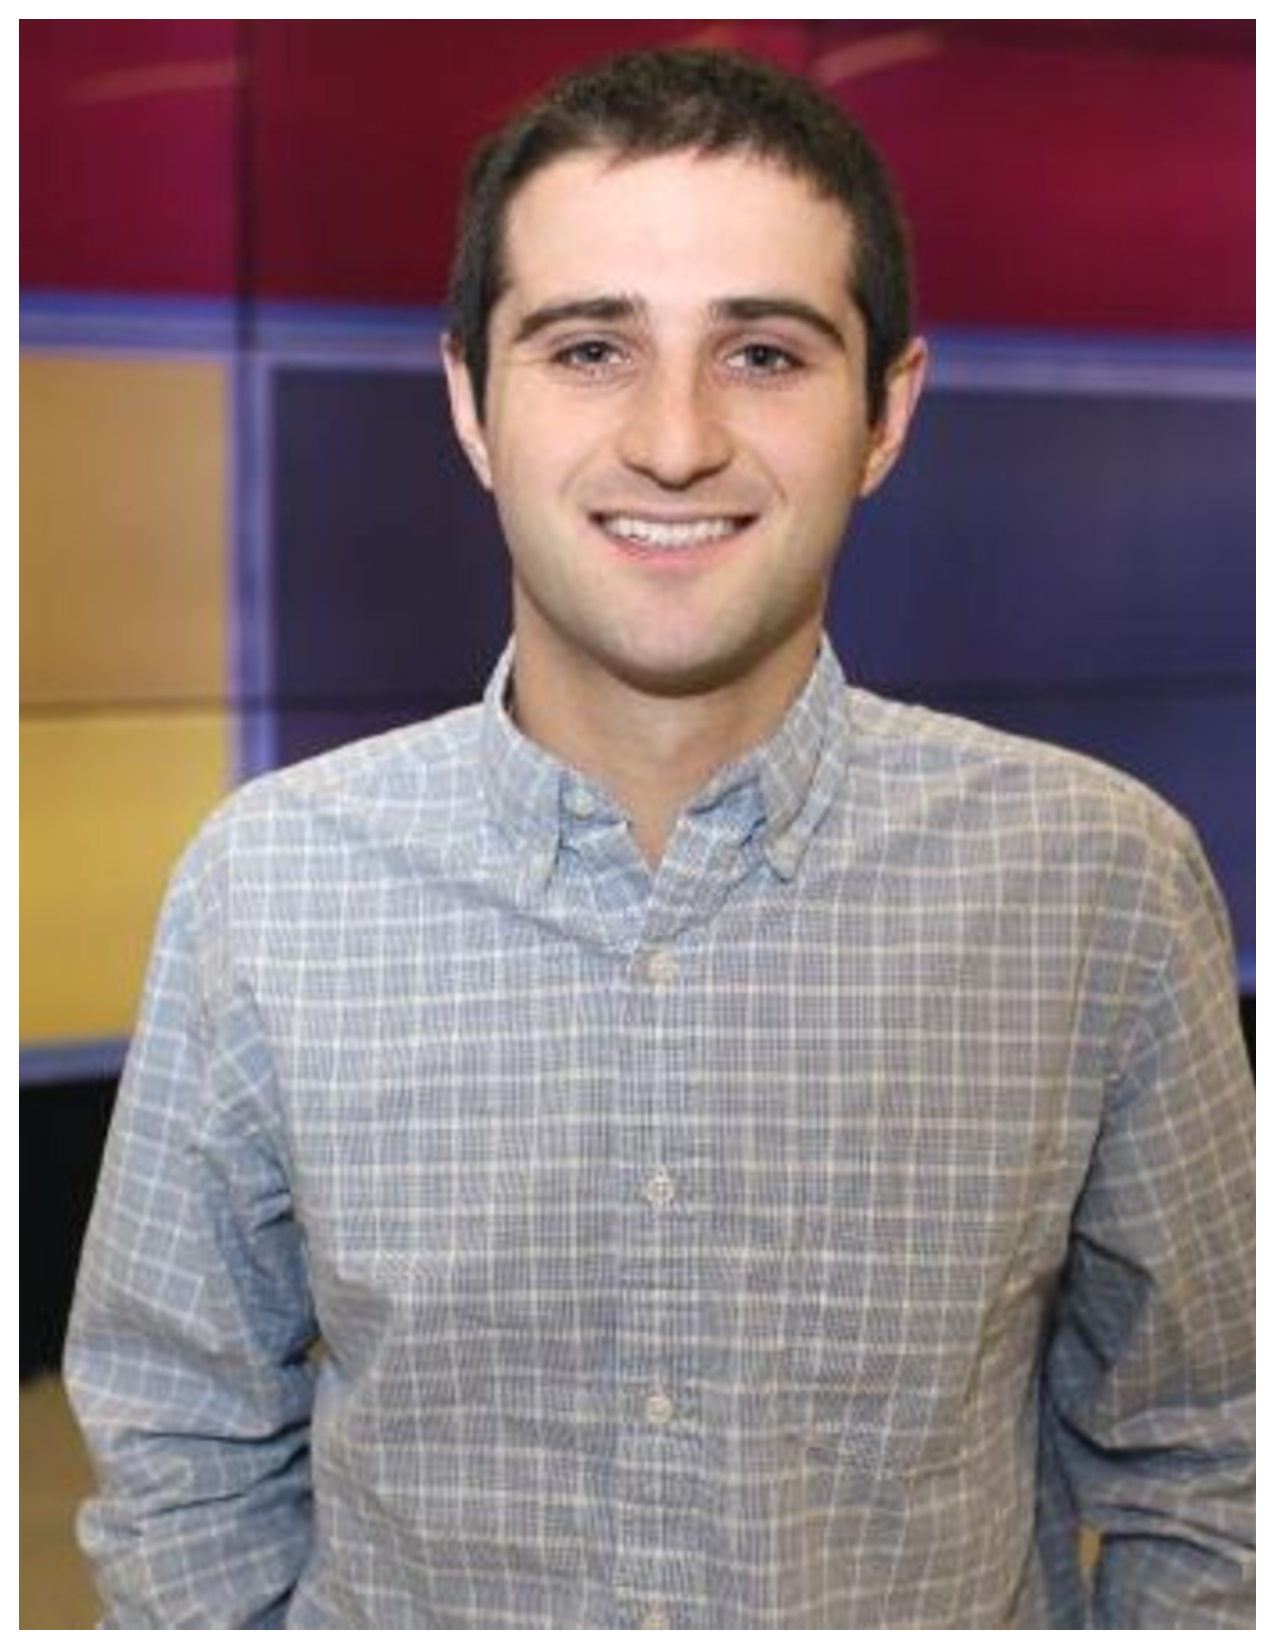
\includegraphics[width=0.25\columnwidth]{images/scott_mcclary}
  \end{wrapfigure}
  \noindent
  {\bfseries Scott McClary} received his BSc (Computer Science) and
  Minor (Mathematics) in May 2016 from Indiana University and will
  receive his MSc (Computer Science) in May 2017 from Indiana
  University. His research interests are within scientific application
  performance analysis on large-scale HPC systems. He will begin
  working as a Software Engineer with General Electric Digital in San
  Ramon, CA in July 2017.
\end{minipage}
\endgroup

\section*{} %used to create more spacing..
\section*{Work Breakdown}
The work on this project was distributed as follows between the
authors:
\begin{description}
\item[Scott McClary.] He completed all of the work for this project
  including researching, deploying, testing and benchmarking the
  Charge Detection Mass Spectrometry research application as well as
  composing this paper.
\end{description}

% Bibliography
\bibliography{references}
\end{document}

